\documentclass[a4paper, 12pt]{article}

\usepackage{wrapfig}
\usepackage{graphicx}
\usepackage{mathtext}
\usepackage{amsmath}
\usepackage{siunitx}
\usepackage{multirow}
\usepackage{rotating}
\usepackage{float}

\usepackage[T1,T2A]{fontenc}

\usepackage[russian]{babel}

\graphicspath{{pictures/}}


\title{\begin{center}Лабораторная работа №1.2.3\end{center}
Определение моментов инерции твердых тел с помощью трифилярного подвеса}
\author{Гёлецян А.Г.}
\date{\today}

\begin{document}
    \pagenumbering{gobble}
    \maketitle
    \newpage
    \pagenumbering{arabic}

    \section{Введение}
    Для измерения моментов инерции сложных тел экспериментальным путем можно воспользоватся
    трифилярным подвесом. Методом несложных вычислении можно найти зависимость периода подвеса от массы и момента инерции иследуемого тела $(1)$. Воспользуемся этой зависимостью для проведения ряда экспериментов, связанных с проверкой теоретической модели.
    \begin{equation}
    I=kmT^2,k=\frac{gRr}{4\pi^2z_0}
    \end{equation}

    \section{Ход работы}
    \subsection{Опыт с 2мя фигурами}

    \paragraph{}
    Для начала проверим для каких углов приближение с использованием малости угла оправдана.
    Несколько измерении показали, что при амплитудах меньше $10^\circ$ период не зависит от
    амплитуды. Соответственно будем придерживатся таких амплитуд.
    \paragraph{}
    Измерим параметры установки для подсчета коэффицента $k$ в формуле $(1)$
    \begin{align*}
        R &= (114.6 \pm 0.5) мм\\
        r &= (30.5 \pm 0.5) мм\\
        m &= (983.2 \pm 0.5) г\\
        z_0 &= (2.14 \pm 0.01) м\\
    \end{align*}
    Из таблиц имеем значение $g=(9,8155 \pm 0.0005)мс^{-2}$ для Москвы. Погрешность $k$ считаем по формуле
    \[\sigma_k=k\sqrt{\left(\frac{\Delta g}{g}\right)^2 +
                     \left(\frac{\Delta r}{r}\right)^2 +
                     \left(\frac{\Delta R}{R}\right)^2 +
                     \left(\frac{\Delta z_0}{z_0}\right)^2}\]
    Подставляя данные получаем
    \[k=(4.06\pm0.07) 10^{-4} м^2с^{-2}\]

    \newpage
    \paragraph{}
    Начнем измерения измерением момента инерции ненагруженной платформы.

    \begin{table}[h!]
    \begin{center}
    \begin{tabular}{|l|r|r|r|}
    \hline
    No &   N &       t, с &         T, с \\
    \hline
    1  &  10 &  44.052 &  4.4052 \\
    2  &  10 &  44.003 &  4.4003 \\
    3  &  10 &  44.005 &  4.4005 \\
    4  &  10 &  43.940 &  4.3940 \\
    5  &  11 &  48.353 &  4.3957 \\
    \hline
    \end{tabular}
    \end{center}
    \end{table}
    Среднее значение $\bar T=4.399$ Случайная погрешность
    $\sigma_T = 0.002с \rightarrow T=(4.399 \pm 0.002)с$. Отсюда \[I_{пф}=kmT^2=(7.7\pm0.1)гм^2\]. Погрешность считалось по формуле
    \[\Delta I = I\sqrt{\left(\frac{\Delta k}{k}\right)^2 +
                     \left(\frac{\Delta m}{m}\right)^2 +
                     \left(2\frac{\Delta T}{T}\right)^2}\]

    \paragraph{}
    Теперь проведем аналогичный опыт, где измерим момент инерции металличесеого кольца
    с характеристиками
    \begin{align*}
    m_{кол} &= (981.7 \pm 0.5) г \\
    r_{внеш} &= (8.45 \pm 0.05) см \\
    r_{внут} &= (7.90 \pm 0.05) см
    \end{align*}

    \begin{table}[h!]
    \begin{center}
    \begin{tabular}{|l|r|r|r|}
    \hline
    No &   N &       t, с &         T, с \\
    \hline
    1  &  10 &  42.459 &  4.2459 \\
    2  &  10 &  42.428 &  4.2428 \\
    3  &  10 &  42.426 &  4.2426 \\
    4  &  10 &  42.385 &  4.2385 \\
    \hline
    \end{tabular}
    \end{center}
    \end{table}
    Из этих данных, аналогично для ненагруженной платформы находим все интересующее.
    \begin{align*}
    T &= (4.242 \pm 0.002)с \\
    I_{пф+кол}&=(14.4 \pm 0.2)гм^2 \\
    I_{кол}&=(6.7 \pm 0.3)гм^2
    \end{align*}

    Теоретической формулой для кольца получаем
    \[I^{теор}_{кол} = m_{кол}\frac{r_{внеш}^2 + r_{внут}^2}{2} = (6.57 \pm 0.05)гм^2\]
    Как видим в пределах погрешности теория соответствует эксперименту.
    \paragraph{}
    Сделаем все то же самое для диска с параметрами
    \begin{align*}
    m_{диск} &= (580.6 \pm 0.5) г \\
    r_{диск} &= (5.75 \pm 0.01) см
    \end{align*}

    \begin{table}[h!]
    \begin{center}
    \begin{tabular}{|l|r|r|r|}
    \hline
    No &   N &       t, с &         T, с \\
    \hline
    1  &  10 &  39.254 &  3.9254 \\
    2  &  10 &  39.221 &  3.9221 \\
    3  &  10 &  39.203 &  3.9203 \\
    4  &  10 &  39.189 &  3.9189 \\
    \hline
    \end{tabular}
    \end{center}
    \end{table}
    Из этих данных получаем


    \begin{align*}
    T &= (3.922 \pm 0.002)с \\
    I_{пф+диск}&=(9.8 \pm 0.2)гм^2 \\
    I_{диск}&=(2.1 \pm 0.3)гм^2
    \end{align*}

    Теоретически получаем
    \[I^{теор}_{диск} = m_{диск}r_{диск}^2 = (1.920 \pm 0.007)гм^2\]
    Как видим в пределах погрешности теория соответствует эксперименту.

    \paragraph{}
    Когда оба тела на платформе.

    \begin{table}[h!]
    \begin{center}
    \begin{tabular}{|l|r|r|r|}
    \hline
    No &   N &       t, с &         T, с \\
    \hline
    1  &  10 &  39.750 &  3.9750 \\
    2  &  10 &  39.873 &  3.9873 \\
    3  &  10 &  39.964 &  3.9964 \\
    4  &  10 &  39.773 &  3.9773 \\
    \hline
    \end{tabular}
    \end{center}
    \end{table}

    \begin{align*}
    T &= (3.984 \pm 0.006)с \\
    I_{пф+общ}&=(16.4 \pm 0.3)гм^2 \\
    I_{общ}&=(8.7 \pm 0.4)гм^2
    I_{диск} + I_{кол}  = (8.8 \pm 0.6)гм^2
    \end{align*}

    Как видим в пределах погрешности момент инерции аддитивен.

    \subsection{Опыт с разрезанным диском}

    Опыт описывать не смысла, сразу приведу данные.

    \begin{table}[h!]
    \begin{center}
    \begin{tabular}{|l|r|r|r|}
    \hline
    h, см   &  T, с & $\sigma_T$, с\\
    \hline
    0.0 &  3.07 &  0.06 \\
    0.5 &  3.08 &  0.05 \\
    1.0 &  3.11 &  0.03 \\
    1.5 &  3.13 &  0.01 \\
    2.0 &  3.16 &  0.01 \\
    2.5 &  3.21 &  0.02 \\
    3.0 &  3.28 &  0.03 \\
    3.5 &  3.35 &  0.02 \\
    4.0 &  3.43 &  0.03 \\
    4.5 &  3.53 &  0.02 \\
    5.0 &  3.63 &  0.03 \\
    5.5 &  3.72 &  0.03 \\
    6.0 &  3.85 &  0.01 \\
    6.5 &  3.97 &  0.02 \\
    7.0 &  4.09 &  0.02 \\
    7.5 &  4.22 &  0.02 \\
    \hline
    \end{tabular}
    \end{center}
    \end{table}
    Ошибка $h \approx 0.1 см$. Теория предсказывает что (здесь $m$ и $I$ это масса и момент инерции платформы, $M$ и $R$ это масса и радиус диска соответственно
    \begin{equation}
        k(m+M)T^2=\frac{MR^2}{2}+Mh^2+I
    \end{equation}

    Нарисуем график $T^2(h^2)$ и сделаем выводы
    \newpage
    \begin{sidewaysfigure}
        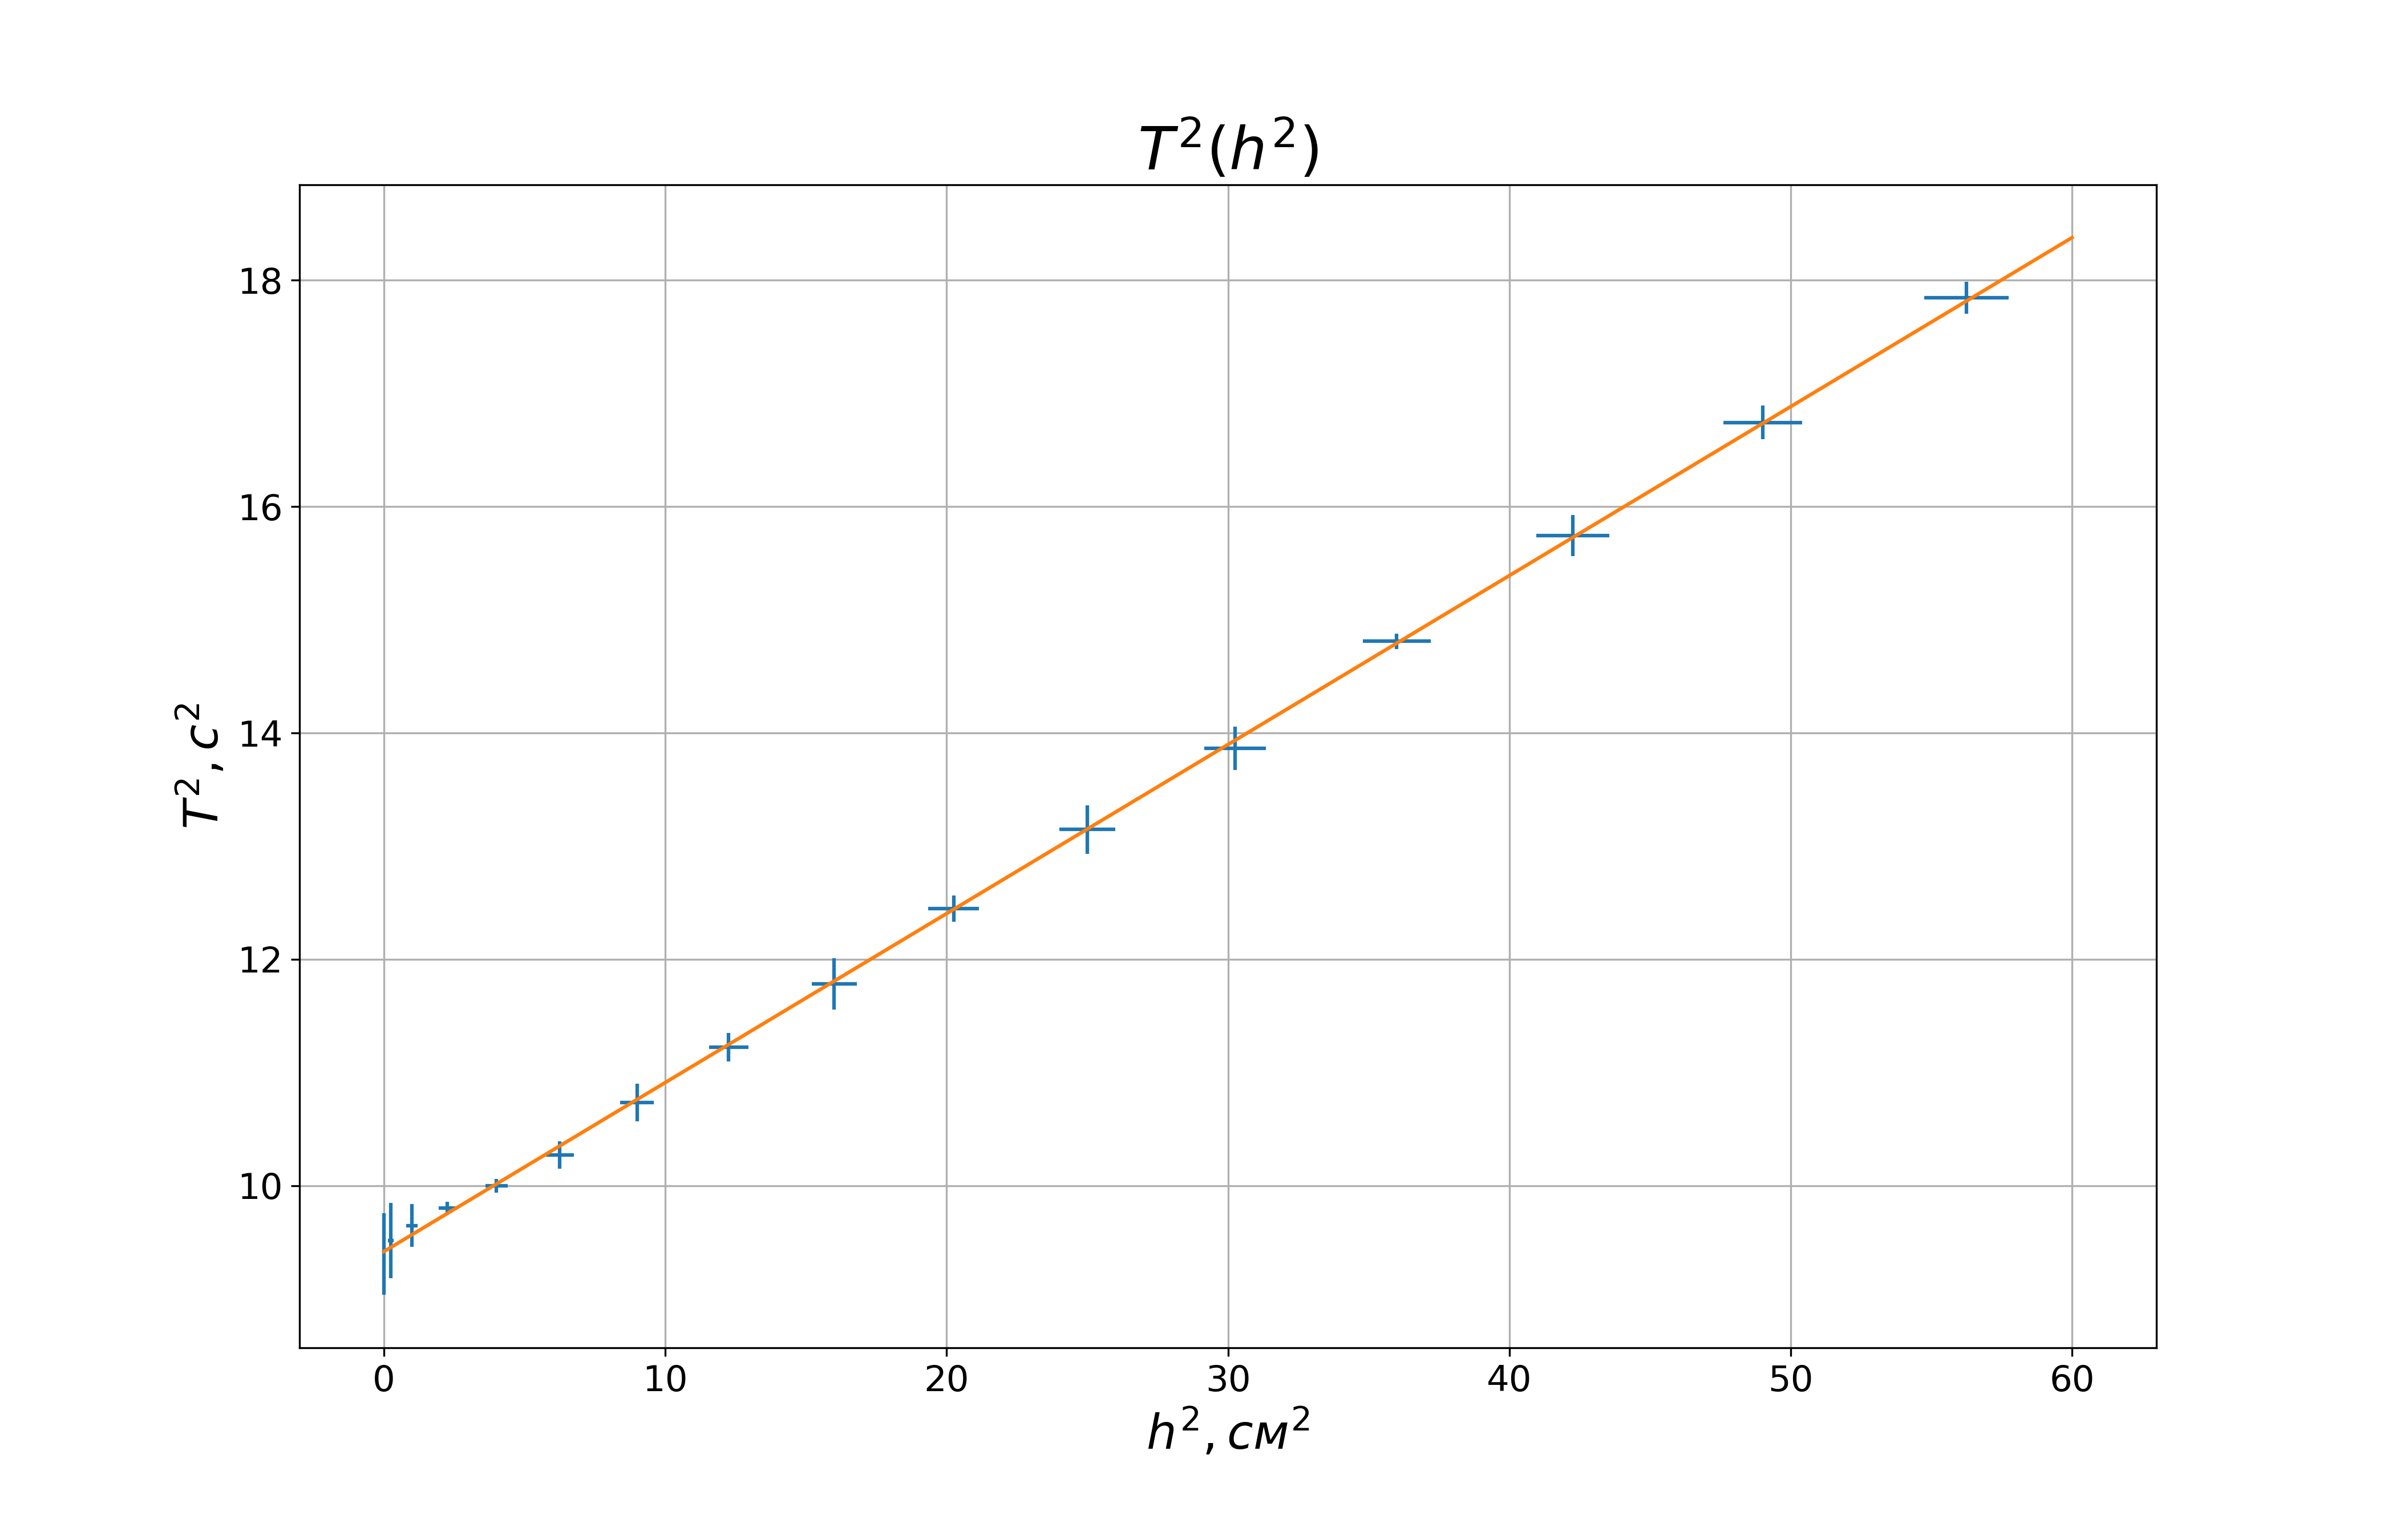
\includegraphics[scale=0.66]{plot.png}
        \caption{График зависимости $T^2(h^2)$}
    \end{sidewaysfigure}
    \newpage

    Формула прямой полученный методом МНК.
    \[T^2 = (0.149 \pm 0.001)с^2см^{-2} h^2 + (9.42 \pm 0.03)с^2\]
    В соответствии с $(2)$ получаем что
    \begin{align*}
    \frac{M}{k(m+M)}&=(0.149 \pm 0.001)с^2см^{-2} &=\alpha \\
    \frac{\frac{MR^2}{2}+I}{k(m+M)}&=(9.42 \pm 0.03)с^2 &=\beta
    \end{align*}

    \begin{align*}
    M&=\frac{km\alpha}{1-k\alpha}\\
    \Delta M &= M\sqrt{\left(\frac{\Delta k}{k}\right)^2 +
                     \left(\frac{\Delta m}{m}\right)^2 +
                     \left(\frac{\Delta \alpha}{\alpha(1-k\alpha)}\right)^2}\\
    M &= (1500 \pm 40)г
    \end{align*}

    Найдем так же момент инерции диска

%     \begin{align*}
    \[I_{диск} =\beta k(m+M) - I\]
    \[\Delta I_{диск} = \sqrt{\left({\Delta I}\right)^2 +
                      \left({k(m+M)\Delta\beta}\right)^2 +
                      \left({\beta(m+M)\Delta k}\right)^2 +
                      \left({\beta k \Delta m})\right)^2 +
                      \left({\beta k \Delta M})\right)^2}
\]
    \[I_{диск}=(1.8\pm0.2)гм^2\]

\end{document}
